%%%%%%%%%%%%%%%%%%%%%%%%%%%%%%%%%%%%%%%%%%%%%%%%%%%%%%%%%%%%%%%%%%%%%%%%%%%%
% AGUtmpl.tex: this template file is for articles formatted with LaTeX2e,
% Modified November 2013
%
% This template includes commands and instructions
% given in the order necessary to produce a final output that will
% satisfy AGU requirements.
%
% PLEASE DO NOT USE YOUR OWN MACROS
% DO NOT USE \newcommand, \renewcommand, or \def.
%
% FOR FIGURES, DO NOT USE \psfrag
%
%%%%%%%%%%%%%%%%%%%%%%%%%%%%%%%%%%%%%%%%%%%%%%%%%%%%%%%%%%%%%%%%%%%%%%%%%%%%
%
% All questions should be e-mailed to latex@agu.org.
%
%%%%%%%%%%%%%%%%%%%%%%%%%%%%%%%%%%%%%%%%%%%%%%%%%%%%%%%%%%%%%%%%%%%%%%%%%%%%
%
% Step 1: Set the \documentclass
%
% There are two options for article format: two column (default)
% and draft.
%
% PLEASE USE THE DRAFT OPTION TO SUBMIT YOUR PAPERS.
% The draft option produces double spaced output.
%
% Choose the journal abbreviation for the journal you are
% submitting to:

% jgrga JOURNAL OF GEOPHYSICAL RESEARCH
% gbc   GLOBAL BIOCHEMICAL CYCLES
% grl   GEOPHYSICAL RESEARCH LETTERS
% pal   PALEOCEANOGRAPHY
% ras   RADIO SCIENCE
% rog   REVIEWS OF GEOPHYSICS
% tec   TECTONICS
% wrr   WATER RESOURCES RESEARCH
% gc    GEOCHEMISTRY, GEOPHYSICS, GEOSYSTEMS
% sw    SPACE WEATHER
% ms    JAMES
% ef    EARTH'S FUTURE
%
%
%
% (If you are submitting to a journal other than jgrga,
% substitute the initials of the journal for "jgrga" below.)

\documentclass[draft,jgrga]{agutexSI}



%%%%%%%%%%%%%%%%%%%%%%%%%%%%%%%%%%%%%%%%%%%%%%%%%%%%%%%%%%%%%%%%%%%%%%%%%
%
%  SUPPORTING INFORMATION TEMPLATE
%
%% ------------------------------------------------------------------------ %%
%
%
%Please use this template when formatting and submitting your Supporting Information.

%This template serves as both a “table of contents” for the supporting information for your article and as a summary of files.
%
%
%OVERVIEW
%
%Please note that all supporting information will be peer reviewed with your manuscript.
%In general, the purpose of the supporting information is to enable authors to provide and archive auxiliary information such as data %tables, method information, figures, video, or computer software, in digital formats so that other scientists can use it.
%The key criteria are that the data:
% 1. supplement the main scientific conclusions of the paper but are not essential to the conclusions (with the exception of
%    including %data so the experiment can be reproducible);
% 2. are likely to be usable or used by other scientists working in the field;
% 3. are described with sufficient precision that other scientists can understand them, and
% 4. are not exe files.
%
%USING THIS TEMPLATE
%
%***All references should be included in the reference list of the main paper so that they can be indexed, linked, and counted as citations.  The reference section does not count toward length limits.
%
%All Supporting text and figures should be included in this document. Insert supporting information content into each appropriate section of the template. %Figures and tables should appear above each caption.  To add additional captions, simply copy and paste each sample caption as needed.

%Tables may be included, but can also be uploaded separately, especially if they are larger than 1 page, or if necessary for retaining table formatting. Data sets, large tables, movie files, and audio files should be uploaded separately, following AGU naming conventions. Include their captions in this document and list the file name with the caption. You will be prompted to upload these files on the Upload Files tab during the submission process, using file type “Supporting Information (SI)”

%IMPORTANT NOTE ON FIGURES AND TABLES
% Placeholders for figures and tables appear after the \end{article} command, after references.
% DO NOT USE \psfrag or \subfigure commands.
%
%  Uncomment the following command to include .eps files
 % \usepackage[dvips]{graphicx}
%
%  Uncomment the following command to allow illustrations to print
%   when using Draft:
%  \setkeys{Gin}{draft=false}
%
% Substitute one of the following for [dvips] above
% if you are using a different driver program and want to
% proof your illustrations on your machine:
%
% [xdvi], [dvipdf], [dvipsone], [dviwindo], [emtex], [dviwin],
% [pctexps],  [pctexwin],  [pctexhp],  [pctex32], [truetex], [tcidvi],
% [oztex], [textures]
%

\usepackage{amsmath} %for help with the bracketed conditional equations
\usepackage{graphicx}
\usepackage{multirow}
\usepackage{mathtools}
\usepackage{chngcntr}
%
%% ------------------------------------------------------------------------ %%
%
%  ENTER PREAMBLE
%
%% ------------------------------------------------------------------------ %%

% Author names in capital letters:
%\authorrunninghead{BALES ET AL.}

% Shorter version of title entered in capital letters:
%\titlerunninghead{SHORT TITLE}

%Corresponding author mailing address and e-mail address:
%\authoraddr{Corresponding author: A. B. Smith,
%Department of Hydrology and Water Resources, University of
%Arizona, Harshbarger Building 11, Tucson, AZ 85721, USA.
%(a.b.smith@hwr.arizona.edu)}

\begin{document}

%% ------------------------------------------------------------------------ %%
%
%  TITLE
%
%% ------------------------------------------------------------------------ %%

%\includegraphics{agu_pubart-white_reduced.eps}


\title{Supporting Information for "Insert Title"}
%
% e.g., \title{Supporting Information for "Terrestrial ring current:
% Origin, formation, and decay $\alpha\beta\Gamma\Delta$"}
%
%DOI: 10.1002/%insert paper number here%

%% ------------------------------------------------------------------------ %%
%
%  AUTHORS AND AFFILIATIONS
%
%% ------------------------------------------------------------------------ %%


%Use \author{\altaffilmark{}} and \altaffiltext{}

% \altaffilmark will produce footnote;
% matching \altaffiltext will appear at bottom of page.

% \authors{A. B. Smith,\altaffilmark{1}
% Eric Brown,\altaffilmark{1,2} Rick Williams,\altaffilmark{3}
% John B. McDougall\altaffilmark{4}, and S. Visconti\altaffilmark{5}}

%\altaffiltext{1}{Department of Hydrology and Water Resources,
%University of Arizona, Tucson, Arizona, USA.}

%\altaffiltext{2}{Department of Geography, Ohio State University,
%Columbus, Ohio, USA.}

%\altaffiltext{3}{Department of Space Sciences, University of
%Michigan, Ann Arbor, Michigan, USA.}

%\altaffiltext{4}{Division of Hydrologic Sciences, Desert Research
%Institute, Reno, Nevada, USA.}

%\altaffiltext{5}{Dipartimento di Idraulica, Trasporti ed
%Infrastrutture Civili, Politecnico di Torino, Turin, Italy.}



%% ------------------------------------------------------------------------ %%
%
%  BEGIN ARTICLE
%
%% ------------------------------------------------------------------------ %%

% The body of the article must start with a \begin{article} command
%
% \end{article} must follow the references section, before the figures
%  and tables.

\begin{article}

%% ------------------------------------------------------------------------ %%
%
%  TEXT
%
%% ------------------------------------------------------------------------ %%



This Supplement provides additional detail about aspects of the analysis included in this study.
%Type or paste your text here. The introduction gives a brief overview of the supporting information. You should include information %about as many of the following as possible (when appropriate):
% 1. a general overview of the kind of data files;
% 2. information about when and how the data were collected or created;
% 3. a general description of processing steps used;
% 4. any known imperfections or anomalies in the data.

%\clearpage
\renewcommand{\thepage}{S\arabic{page}}  
\renewcommand{\thesection}{S\arabic{section}}   
\renewcommand{\thetable}{S\arabic{table}}   
\renewcommand{\thefigure}{S\arabic{figure}}
\setcounter{figure}{0}

\section{Metropolis Evaluation}
\counterwithin{figure}{section} %reset figure numbering

The metropolis algorithm was evaluated for 450,000 iterations, with the first 10,000 discarded as ``burnin" iterations, during which the model was experiencing transient behavior. Such a large number of iterations allows for convergence of all parameters to their best solutions. Our method is based on a markov chain, such that the proposed parameter values for each iteration depend on the values from the last accepted iteration according to:
\begin{equation}\label{eqn:proposal}
\begin{split}
delta&=Range(Prior) \\
Proposal_i&=Accepted_{i-1} + dp \cdot (0.5-rand) \cdot delta; 
\end{split}\tag{S1}
\end{equation}
where $delta$ is the range allowed by the uniform prior for each parameter and $rand$ is a random number between 0 and 1. $Proposal_i$ is the value of a parameter for iteration $i$ and $Accepted_{i-1}$ is the previous value of that parameter accepted by the algorithm. To more efficiently explore parameter space, proposed parameters were selected with step sizes $dp_{Age}$ = 0.1 and $dp_{TWTT}$ = 0.1 for those parameters associated with each likelihood in Equation~\ref{eqn:bigproblem}.

The evaluation of the two likelihood functions (i.e. ``cost") are independently accepted according to each function's metropolis probability during each iteration. The accepted solutions for each cost, depth, and age are shown in Figure~\ref{fig:cost}. As seen in the figure, these cost values show little trend aside from occasional positive departures from the mean as the model explores parameter space. 

\begin{figure*}[ht]
%\begin{center}
\centering
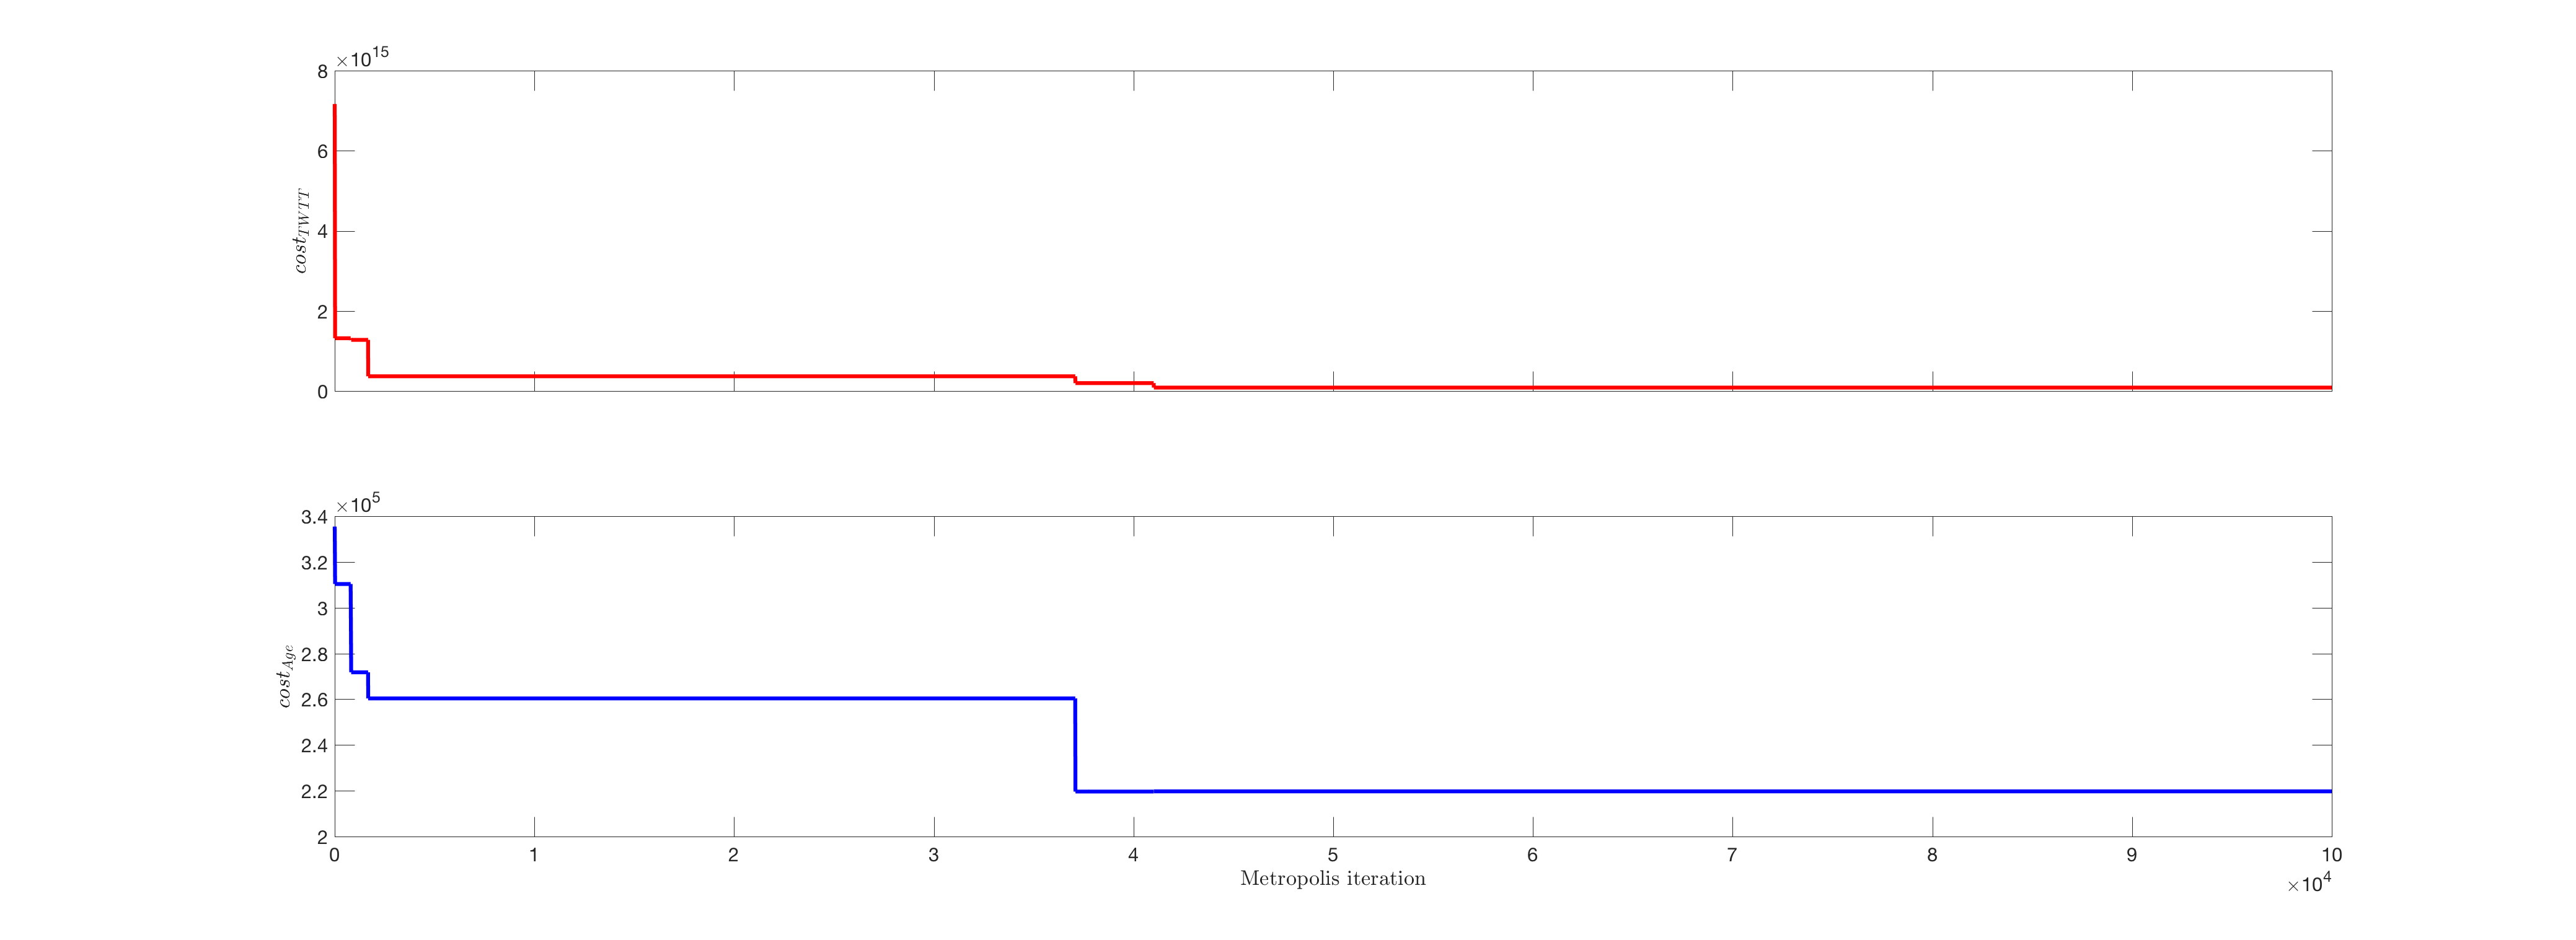
\includegraphics[scale=0.4]{../analysis/figures/cost}
%\captionsetup{width=.9\textwidth}
\caption[]{Cost of the age and depth likelihood functions at each accepted iteration.}
%\end{center}
\label{fig:cost}
\end{figure*}





\section{Regularization}\label{sec:regularization}
\counterwithin{figure}{section} %reset figure numbering

Sampling accumulation rate parameters along the depth profile is inefficient and problematic because many proposed solutions are unrealistically variable. We expect the mean accumulation rate over time (and therefore depth) changes slowly and continuously. To improve our accumulation rate solutions, we regularize the likelihood of reflector age. A regularization parameter is added to the age cost term which punishes proposed accumulation rate profiles which are highly variable relative to a solution computed with no regularization and smoothed over a moving 600-m depth window. This window size is chosen because it is the smallest interval over which the data can be smoothed given the 200-m bin size of the accumulation rate parameters. 

The regularization term, $r$ is the ratio of the variance of a proposed set of accumulation rates to the variance of the smoothed, non-regularized accumulation rate profile. Values of the regularization term for accepted parameter solutions are shown in Figure~\ref{fig:reg}. The regularization is weighted as $r^6$ when included in the calculation of the age cost (Equation~\ref{eqn:loglikeage}) to sufficiently reduce variability in the accumulation rate profile. 


\begin{figure*}[ht]
%\begin{center}
\centering
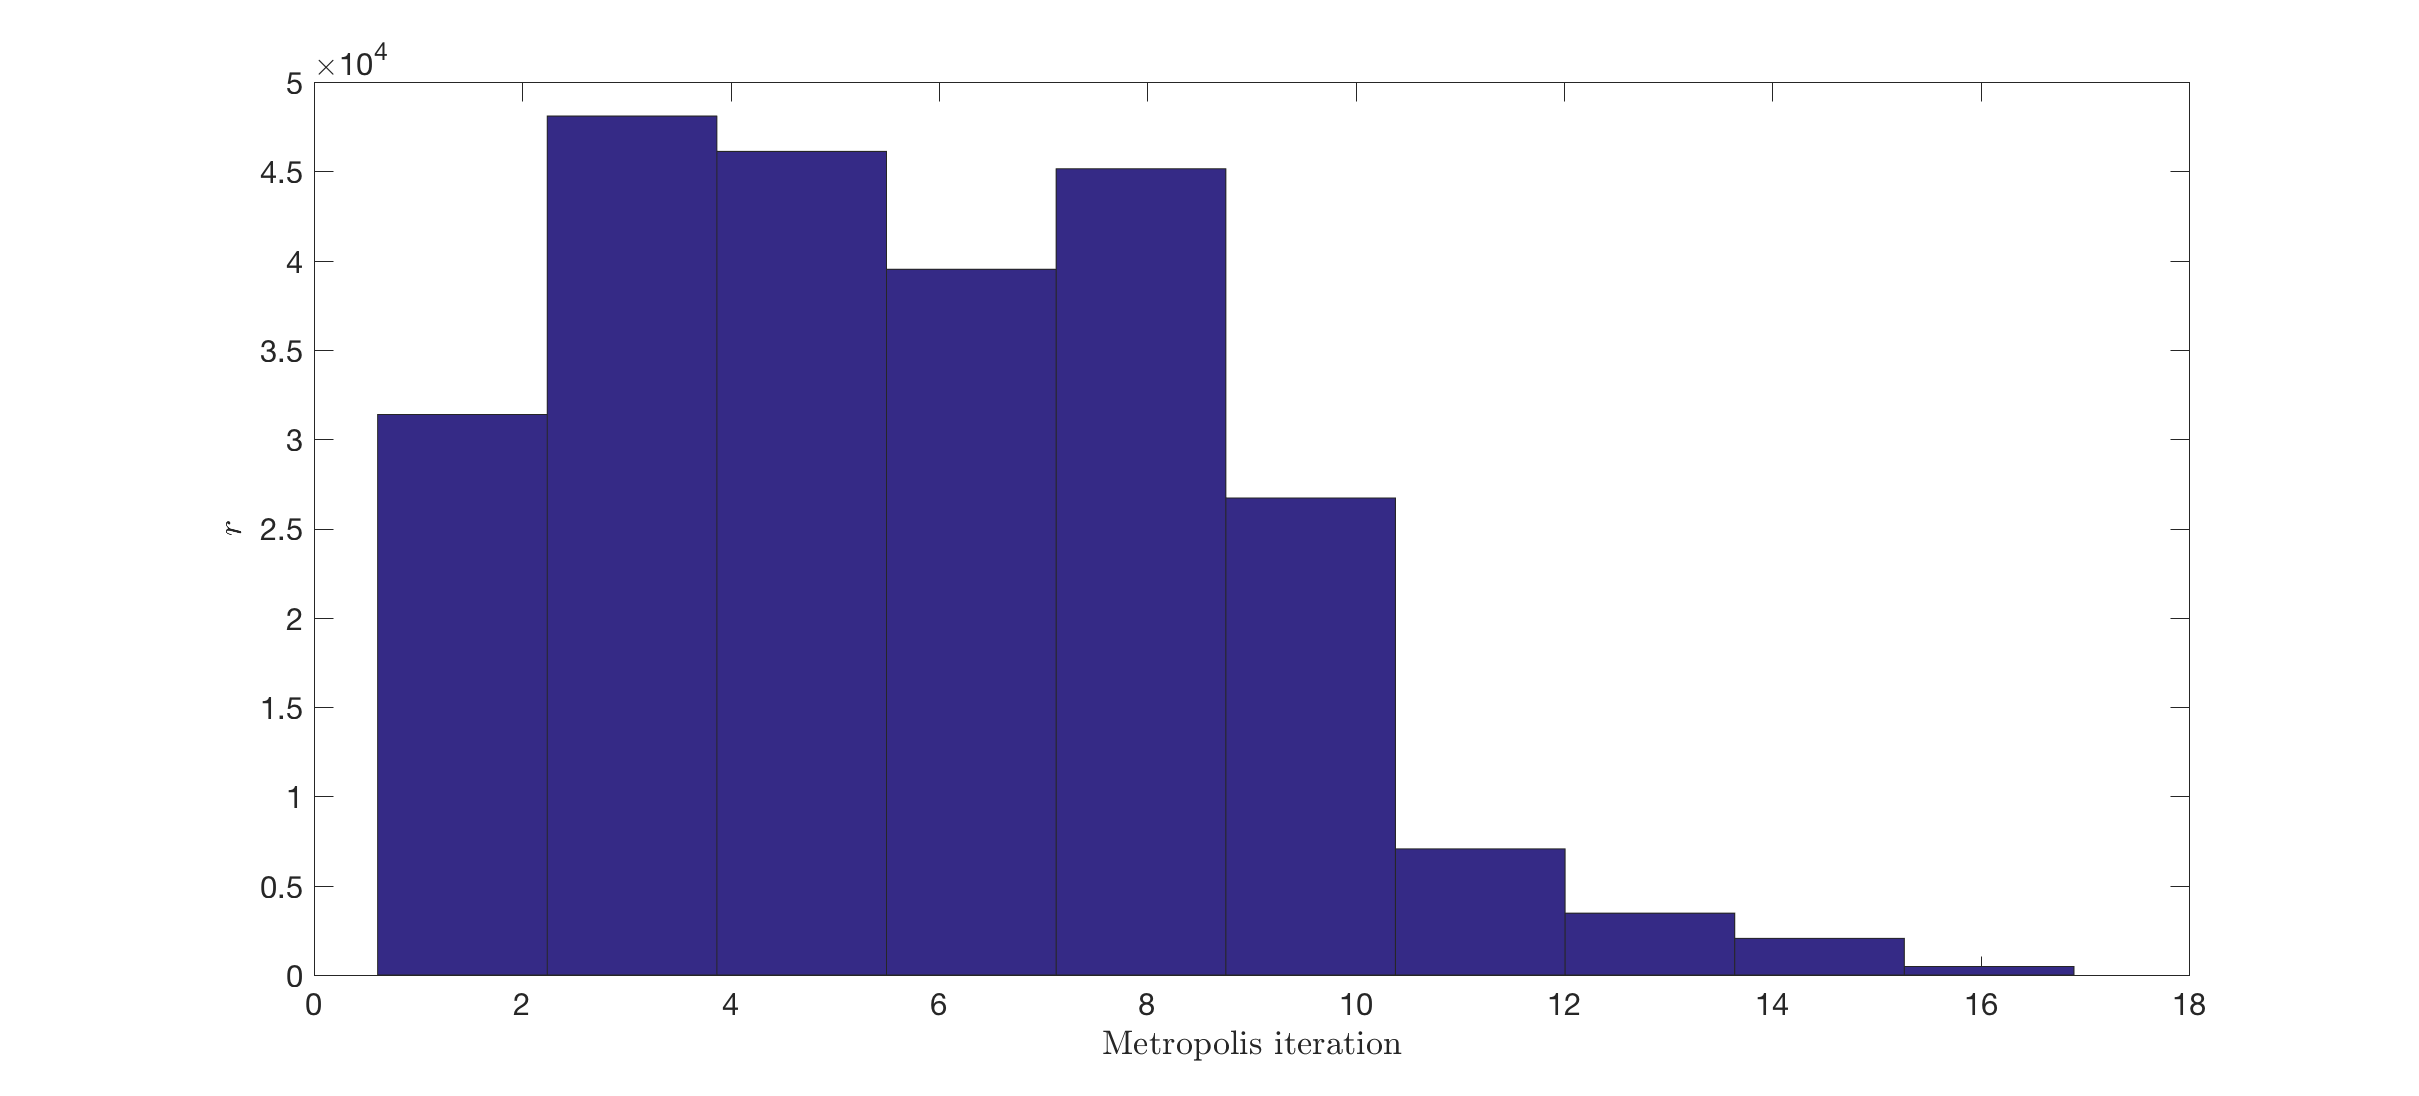
\includegraphics[scale=0.4]{../analysis/figures/regularization}
%\captionsetup{width=.9\textwidth}
\caption[]{Values of the regularization parameter at each accepted metropolis iteration.}
%\end{center}
\label{fig:reg}
\end{figure*}








\section{Estimating TWTT uncertainty}\label{sec:sigmatwtt}
\counterwithin{figure}{section} %reset figure numbering
To estimate $\sigma_{TWTT}$ in Equation~\ref{eqn:loglikeage}, we assume a perfect model then perturb it with errors consistent what we expect to find in the data. We assume the depth errors can be described by a gaussian distribution which results in the following relationship between the cost, degrees of freedom, and $\sigma_{TWTT}$ \citep{jackson&huerta2016}.


\begin{equation}
\frac{1}{\sigma_{TWTT}}= \frac{\sqrt{k_e/2}}{\sigma_{{E_m}^*}}\tag{S2}
\end{equation}
Here $k_e$ is the effective number of degrees of freedom and ${E_m}^*$ represents the perfect model of TWTT which is perturbed with errors consistent with what we expect to find in the radar observations. For simplicity, we assume $k_e$ is the same as the number of reflectors for which we invert.

This method makes use of the ``perfect model":
\begin{equation}
cost^*_{TWTT} = \frac{\sum_{j = z}[TWTT_m(z) - \overline{TWTT_m}(z)]^2}{2}
\end{equation}


% \section{Byrd ice core volcanic chronology}\label{sec:volcanic}

% Table of those points from the 50ka record used (i.e. ones with unique depths at 1-m model resolution)





\section{Degrees of freedom and parameter correlation}\label{sec:ke}
\counterwithin{figure}{section} %reset figure numbering

As we invert for model parameter values, we anticipate the data points used to constrain our likelihood functions -- sourced from radar observations and a Byrd ice core volcanic chronology -- are not independent of one another. As a result, we expect the number of degrees of freedom to be less than the number of data points available. While we do not know the number of effective degrees of freedom, $k_e$, we explore the sensitivity of our results to our choice of $k_e$ (Figure~\ref{fig:ke}). We find that our choice does not significantly impact the mean estimates of age or depth for our radar reflectors. In lieu of more information about the degrees of freedom, we choose to assume $k_e = \frac{N_{data}}{2} = 30.5$ because convergence on the accumulation rates are strong and the rate at which the algorithm finds solutions is reasonable. 

\begin{figure*}[ht]
\begin{center}
%\centering
\makebox[\textwidth][c]{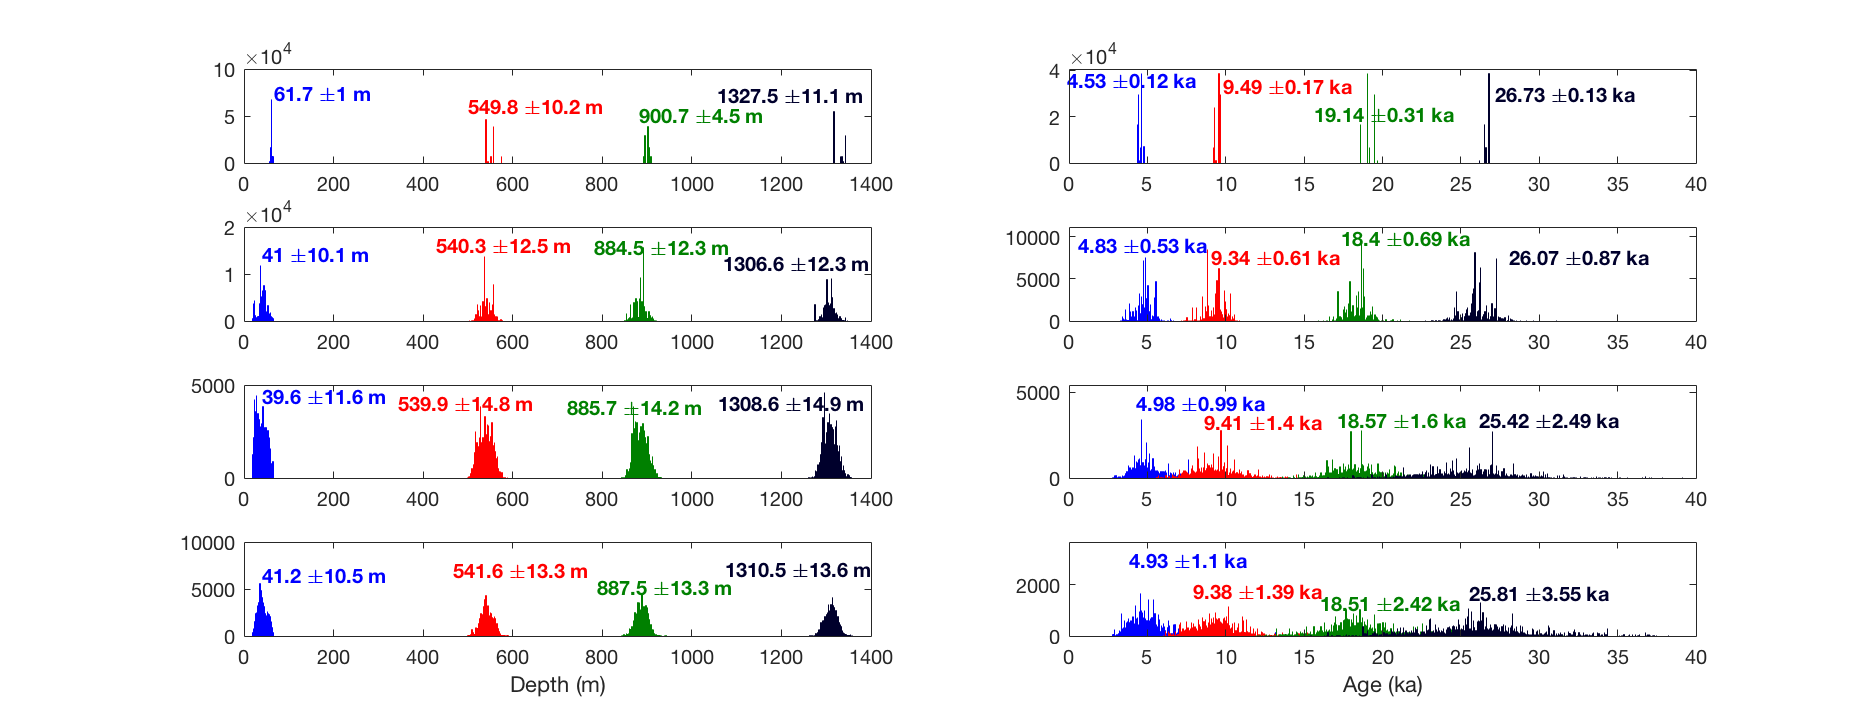
\includegraphics[scale=0.35]{../analysis/figures/keCompare_tweaked}}
%\captionsetup{width=.9\textwidth}
\caption[scale=0.3]{Comparison of results for reflector age and depth assuming a range of $k_e$ values. All agree to within uncertainty.}
\end{center}
\label{fig:ke}
\end{figure*}

Figure~\ref{fig:flowparamconvergence} shows the results of inverting for several model parameters in this problem, including flow parameters such as $q$ as well as ice property parameters such as $v_{ice}$. The results show the parameters are not correlated with one another and do seem to convergence to most-likely solutions.

\begin{figure*}[ht]
%\begin{center}
\centering
\makebox[\textwidth][c]{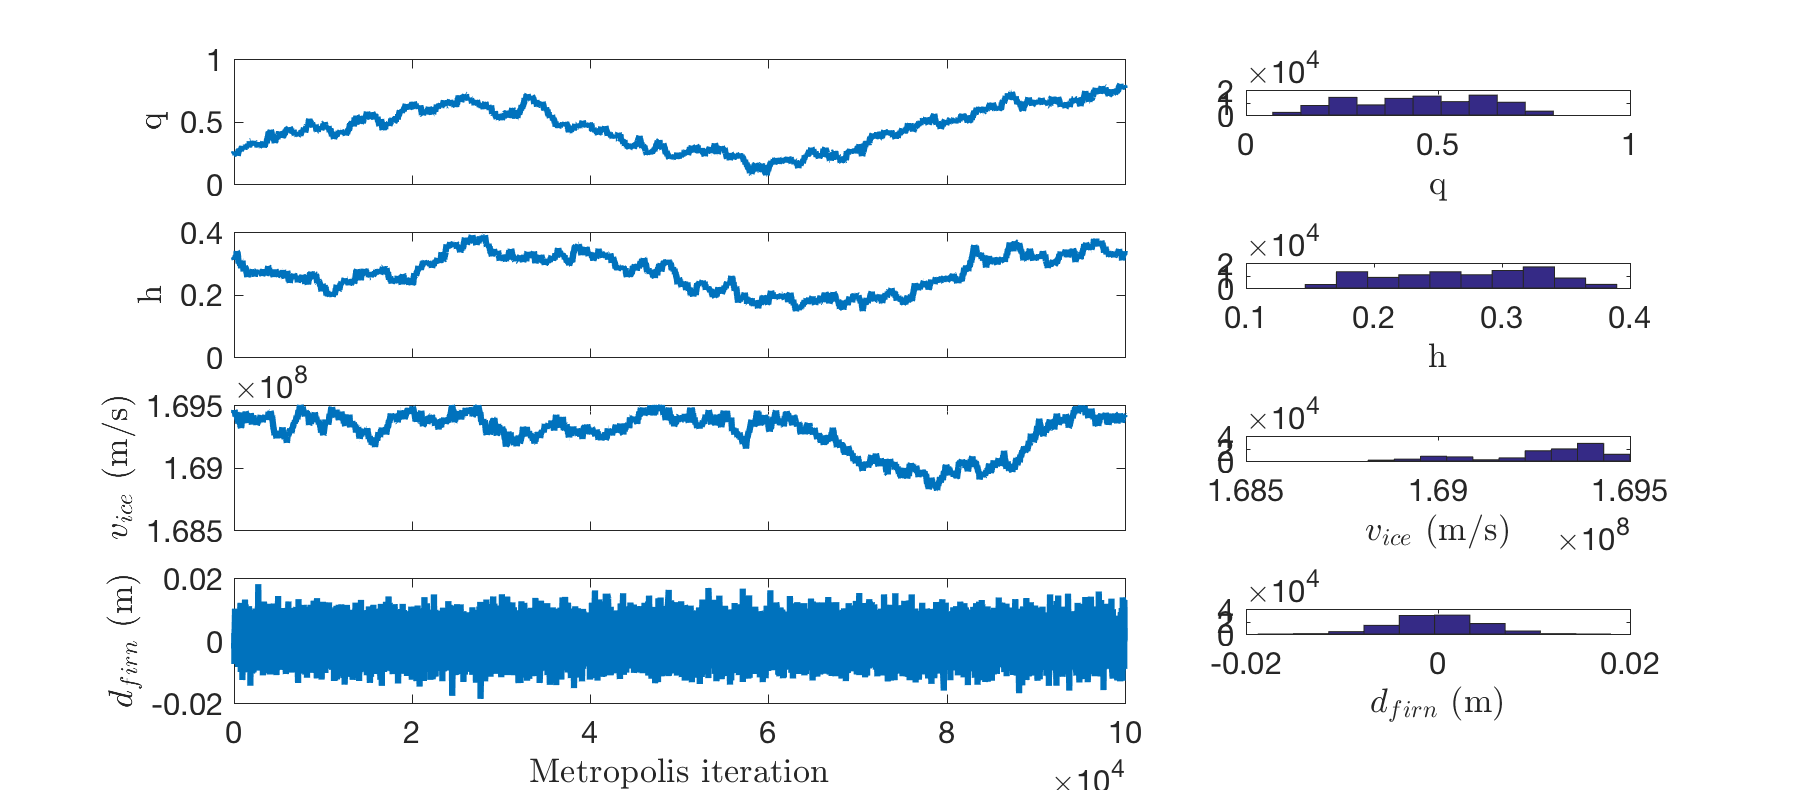
\includegraphics[scale=0.4]{../analysis/figures/convergence1}}
%\captionsetup{width=.9\textwidth}
\caption[]{Left: Flow parameter values at each accepted Metropolis iteration for parameters $q$ (top), $h$, $v_{ice}$, and $d_{firn}$ (bottom). The parameter values do not appear correlated Right: Histograms of the parameter values shown in the left column. Histograms show the parameter values converging.}
%\end{center}
\label{fig:flowparamconvergence}
\end{figure*}

Accumulation rate is divided into 10 parameters, each covering a depth bin of $\sim$200 m. This allows for variation in the accumulation rate over time, as expected. The resulting accumulation rate profiles are shown in Figure~\ref{fig:accumdepth}. As discussed elsewhere in the Supplemental Information, these profiles have been regularized to preferentially select those which do not exhibit unrealistic variability. In Figure~\ref{fig:accumdepth}, they have been additionally sorted by cost to demonstrate the relative quality of the accepted solutions.

\begin{figure*}[ht]
%\begin{center}
\centering
\makebox[\textwidth][c]{\includegraphics[scale=0.4]{../analysis/figures/accumdepthSorted}}
%\captionsetup{width=.9\textwidth}
\caption[]{Accumulation rate as a function of ice depth colored by cost value for the estimated parameter values. (Accumulation rate series associated with lower cost are expected to be solutions.) Accumulation rate is estimated in 10 depth bins at $\sim$200 m depth intervals. Transitions between these intervals have been smoothed in this figure for each of viewing.}
%\end{center}
\label{fig:accumdepth}
\end{figure*}

To further explore the accumulation rate solutions, we look at the accepted parameter values and their convergence over all iterations. As seen in the right side of Figure~\ref{fig:accumconvergence}, the accumulation rate solutions do not converge as readily as other parameters, leaving wider distributions exhibiting more uncertainty in our estimates of accumulation rate. This may mean that our priors play an important role in estimating the value of accumulation rate and therefore the result could be improved with a more informative prior. This is particularly true at the bottom of the ice column, where neither volcanic chronology data nor radar data is available to constrain the accumulation rate.

We see correlation between some accumulation rate parameters (left side of Figure~\ref{fig:accumconvergence}). This may indicate we could have combined these accumulation rate depth bins. Figure~\ref{fig:accumCorrelation} shows a correlation matrix between pairs of accumulation rate parameters. Along the diagonal are histograms of each accumulation rate parameter. Pairs of accumulation rate parameters to not tend to be very correlated and only one pair of accumulation rate parameters has $R^2 > 0.5$. In general, $R^2$ values are highest between accumulation rates in the lower part of the ice column, where parameter values are more difficult to constrain due to a lack of data and flatter age-depth profile.


\begin{figure*}[ht]
%\begin{center}
\centering
\makebox[\textwidth][c]{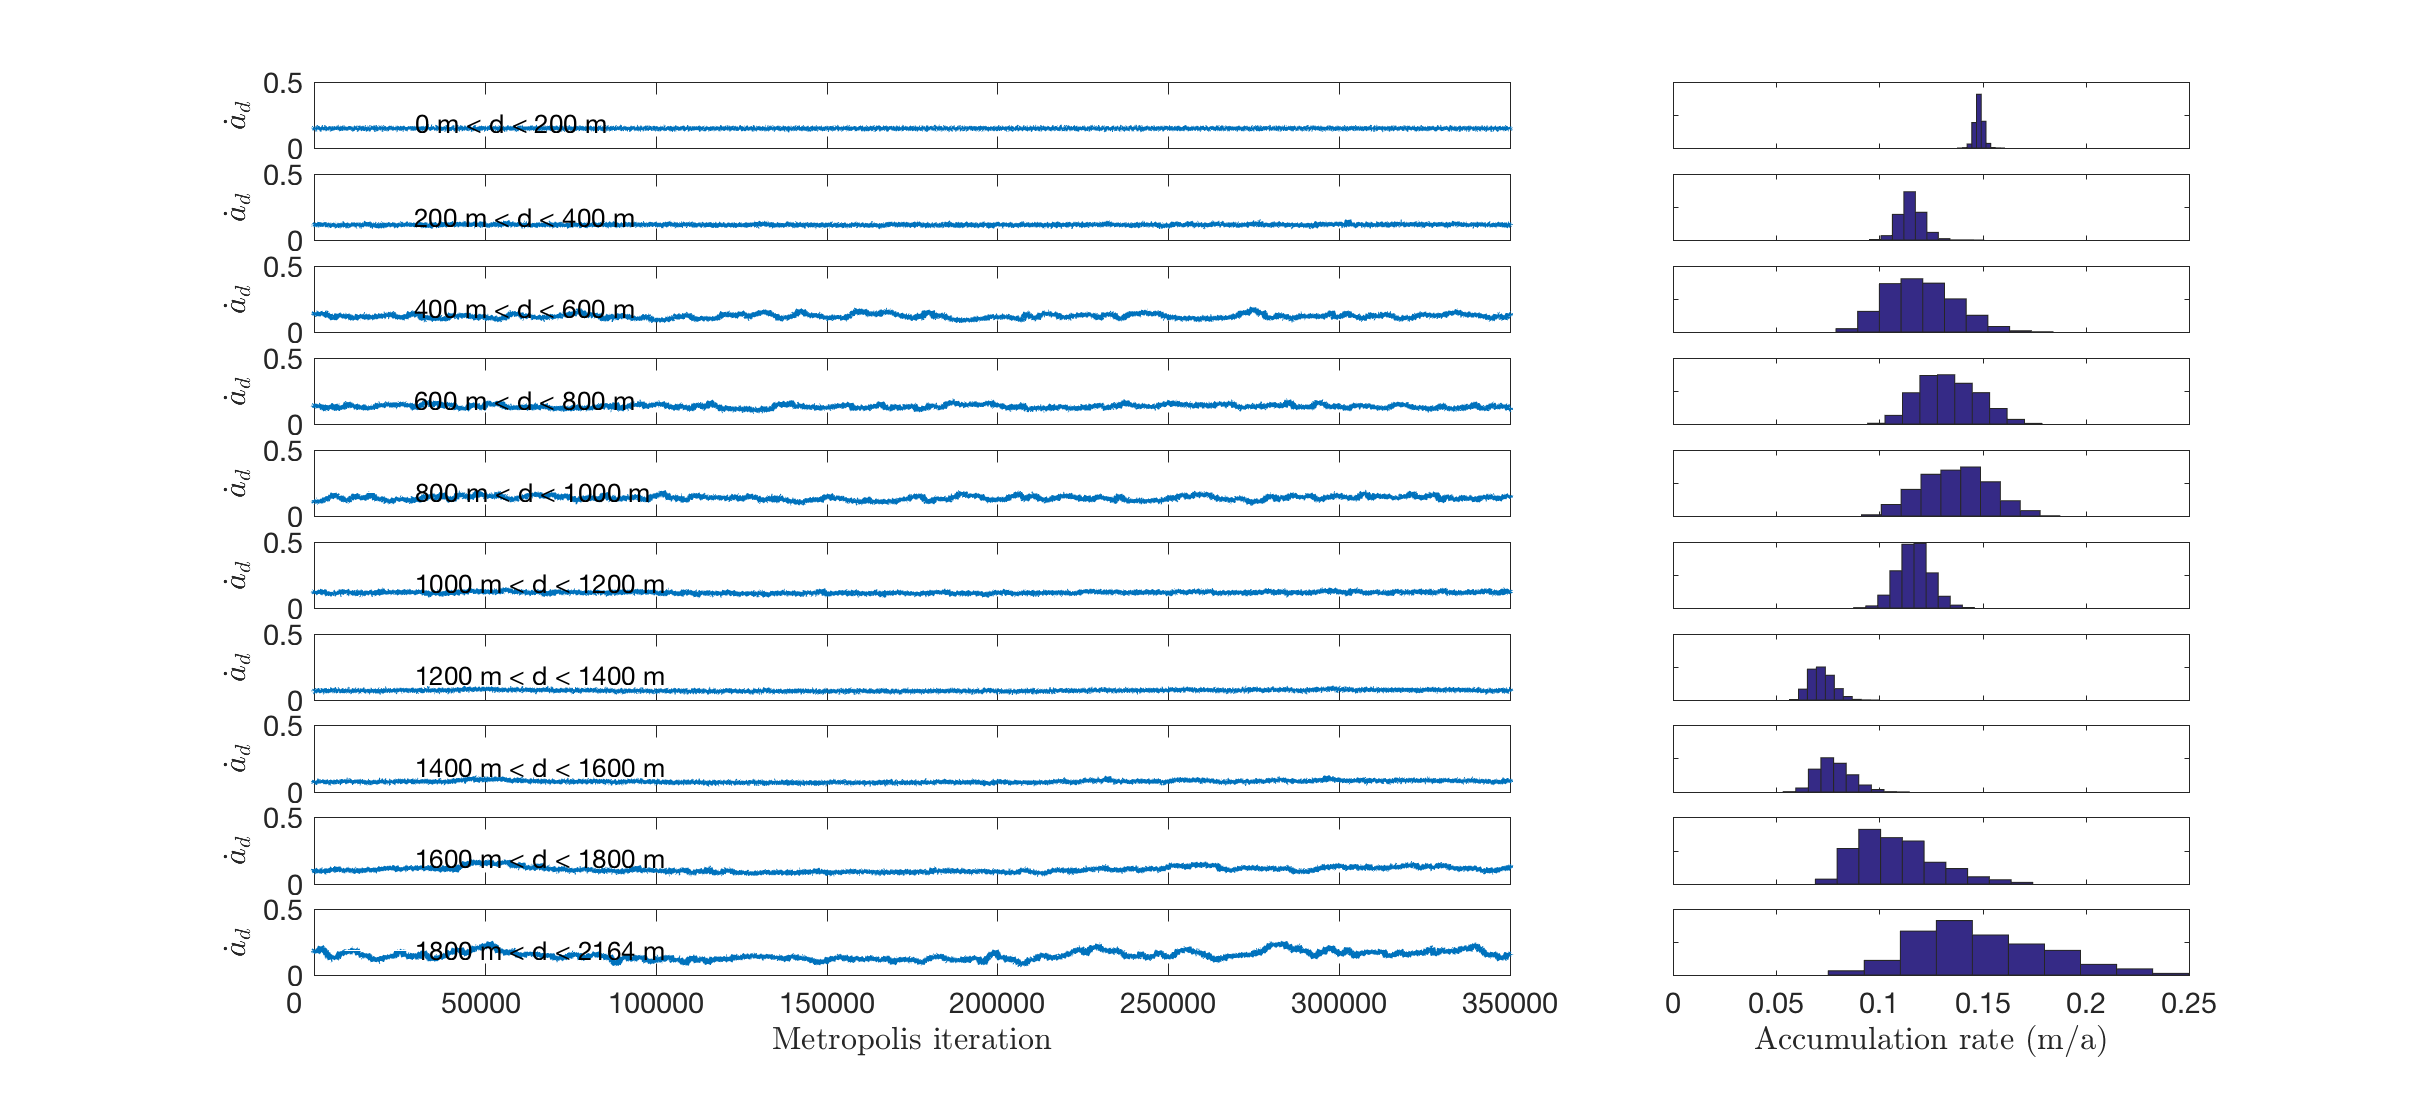
\includegraphics[scale=0.4]{../analysis/figures/convergence2}}
%\captionsetup{width=.9\textwidth}
\caption[]{Left: Values of each accumulate rate parameter (in each of 10 depth bins, shallowest at top). Right: Histograms of the parameter values at left. Certain depth bins appear to be correlated and the histograms of values are wider, indicating the accumulation rate parameters are slower to converge and more uncertain.}
%\end{center}
\label{fig:accumconvergence}
\end{figure*}

\begin{figure*}[ht]
%\begin{center}
\centering
\makebox[\textwidth][c]{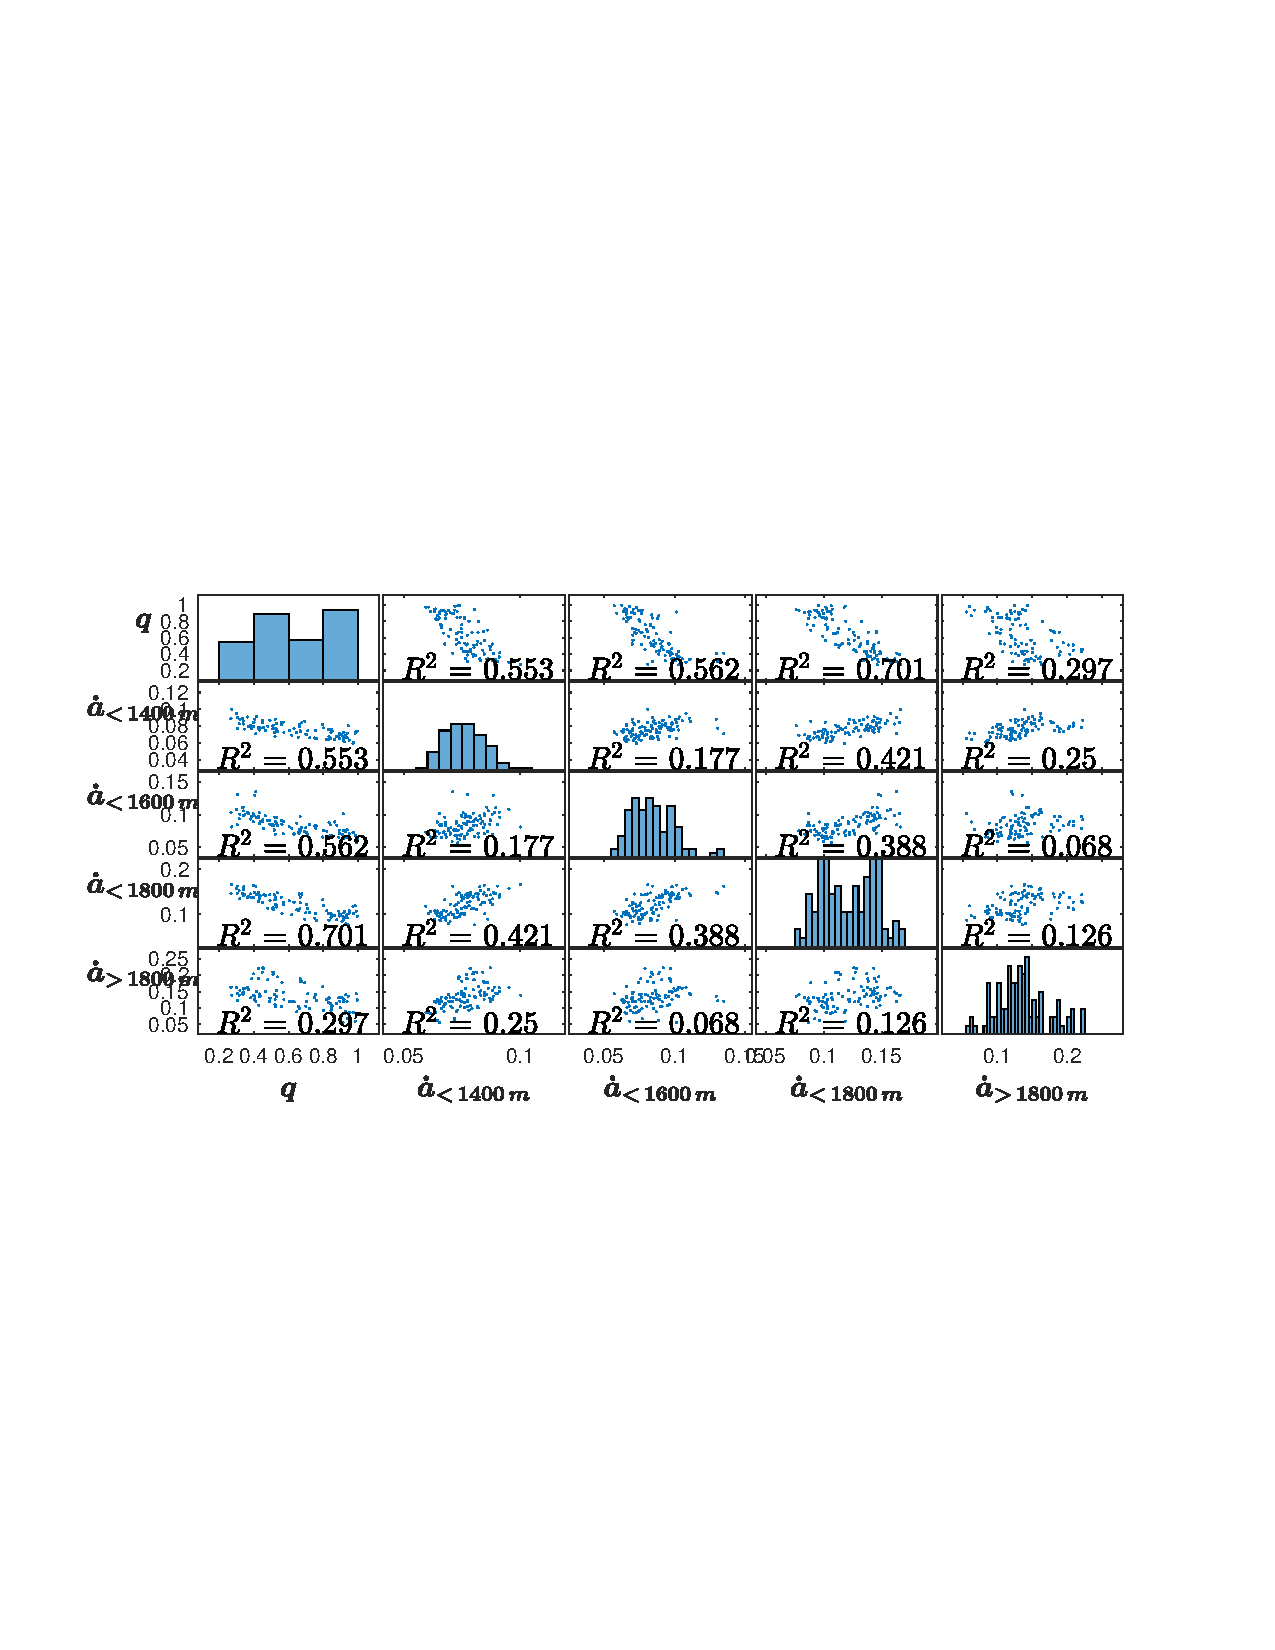
\includegraphics[scale=0.4]{../analysis/figures/accumCorrelation}}
%\captionsetup{width=.9\textwidth}
\caption[]{Correlation of each accumulation rate parameter with every other accumulation rate parameter. Histograms of each accumulation rate are shown along the diagonal. Pairs of parameters with $R^2 > 0.5$ have their correlation coefficients shown in red.}
%\end{center}
\label{fig:accumCorrelation}
\end{figure*}


% Convergence of the reflector depths is shown in Figure~\ref{fig:depthconvergence}.


% \begin{figure*}[ht]
% %\begin{center}
% \centering
% \makebox[\textwidth][c]{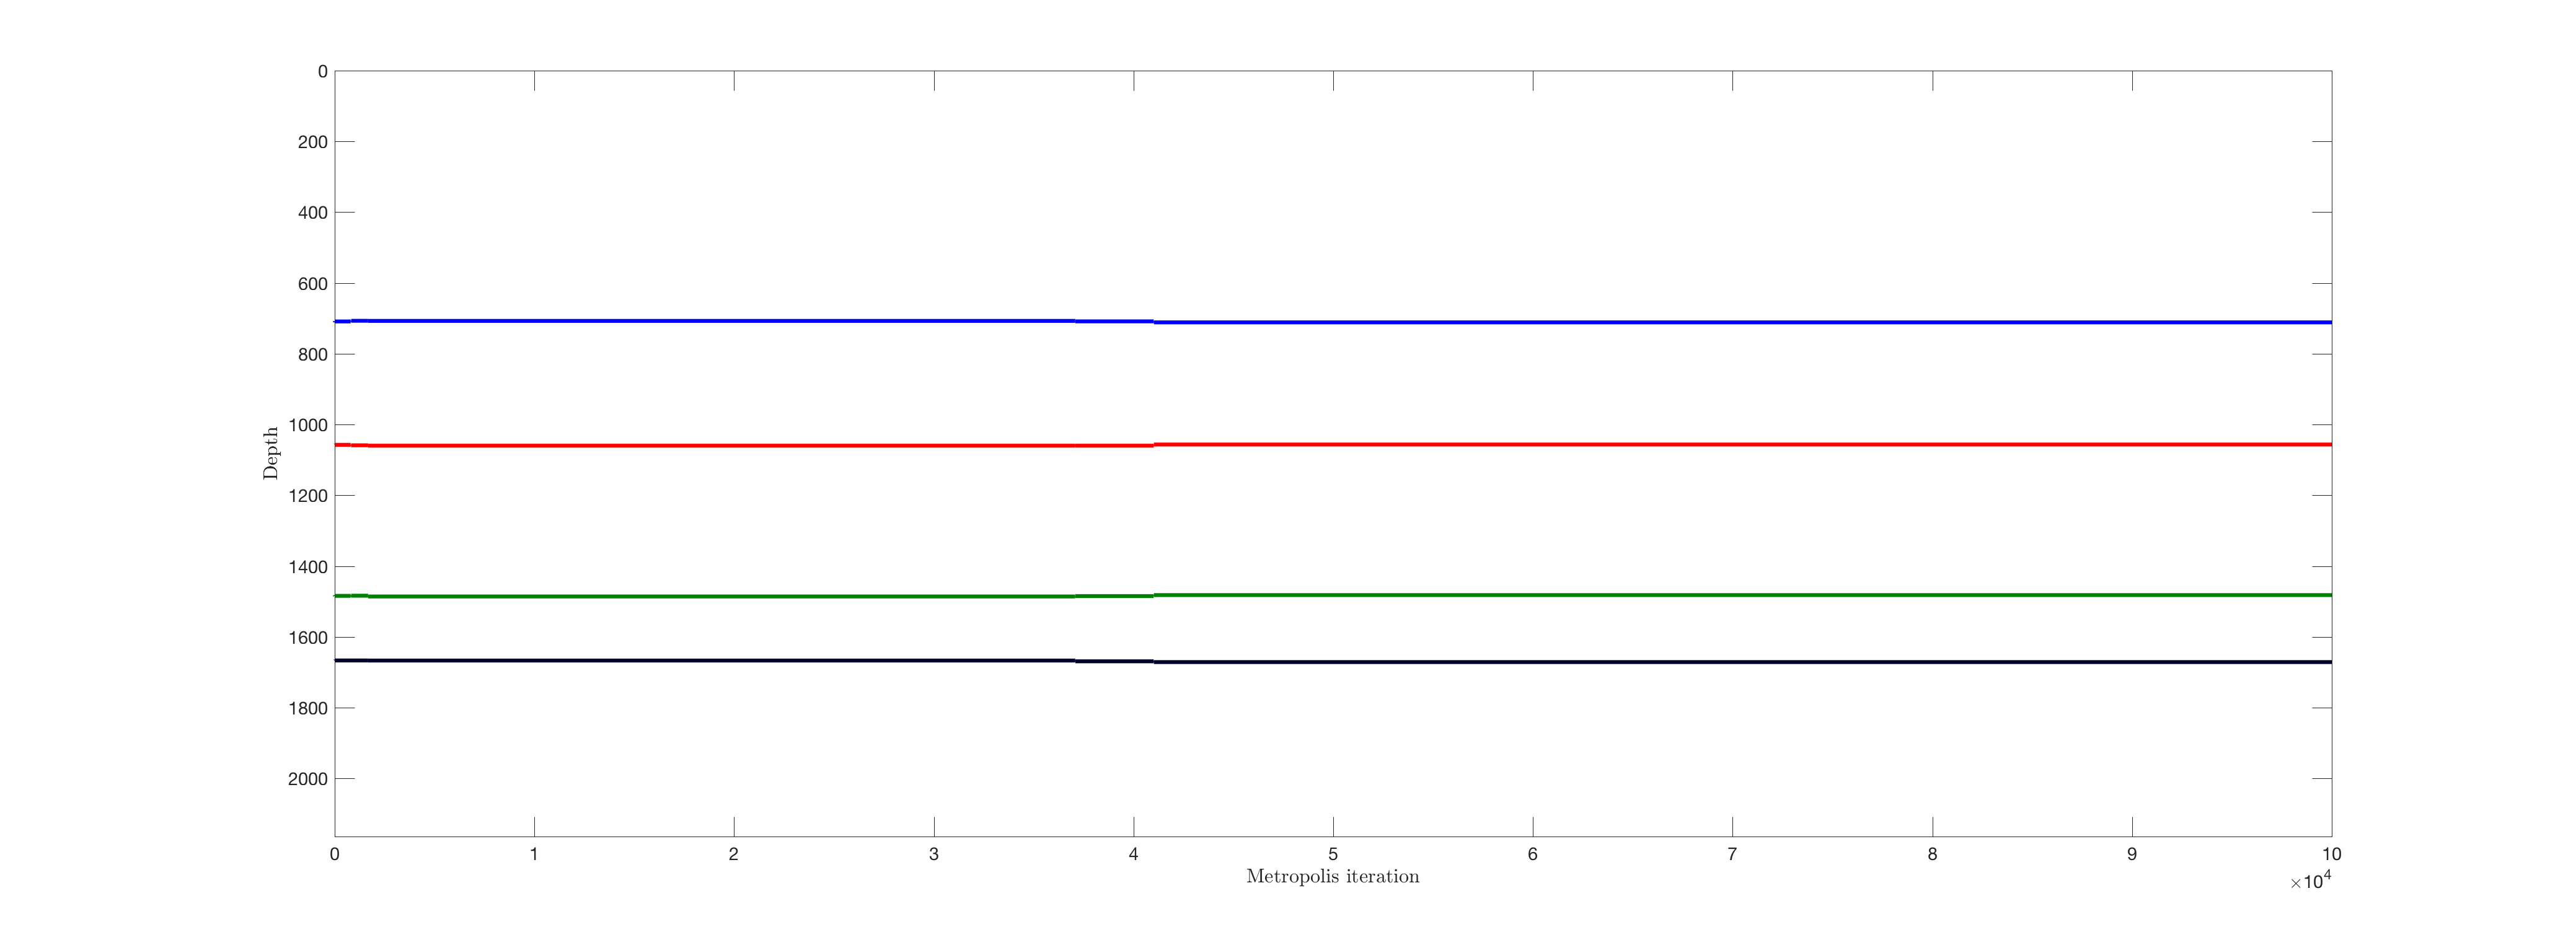
\includegraphics[scale=0.4]{../analysis/figures/convergence3}}
% %\captionsetup{width=.9\textwidth}
% \caption[]{Reflector depth values at each accepted metropolis iteration.}
% %\end{center}
% \label{fig:depthconvergence}
% \end{figure*}



% \section{Firn Correction}

% \begin{figure*}[h]
% %\begin{center}
% \centering
% 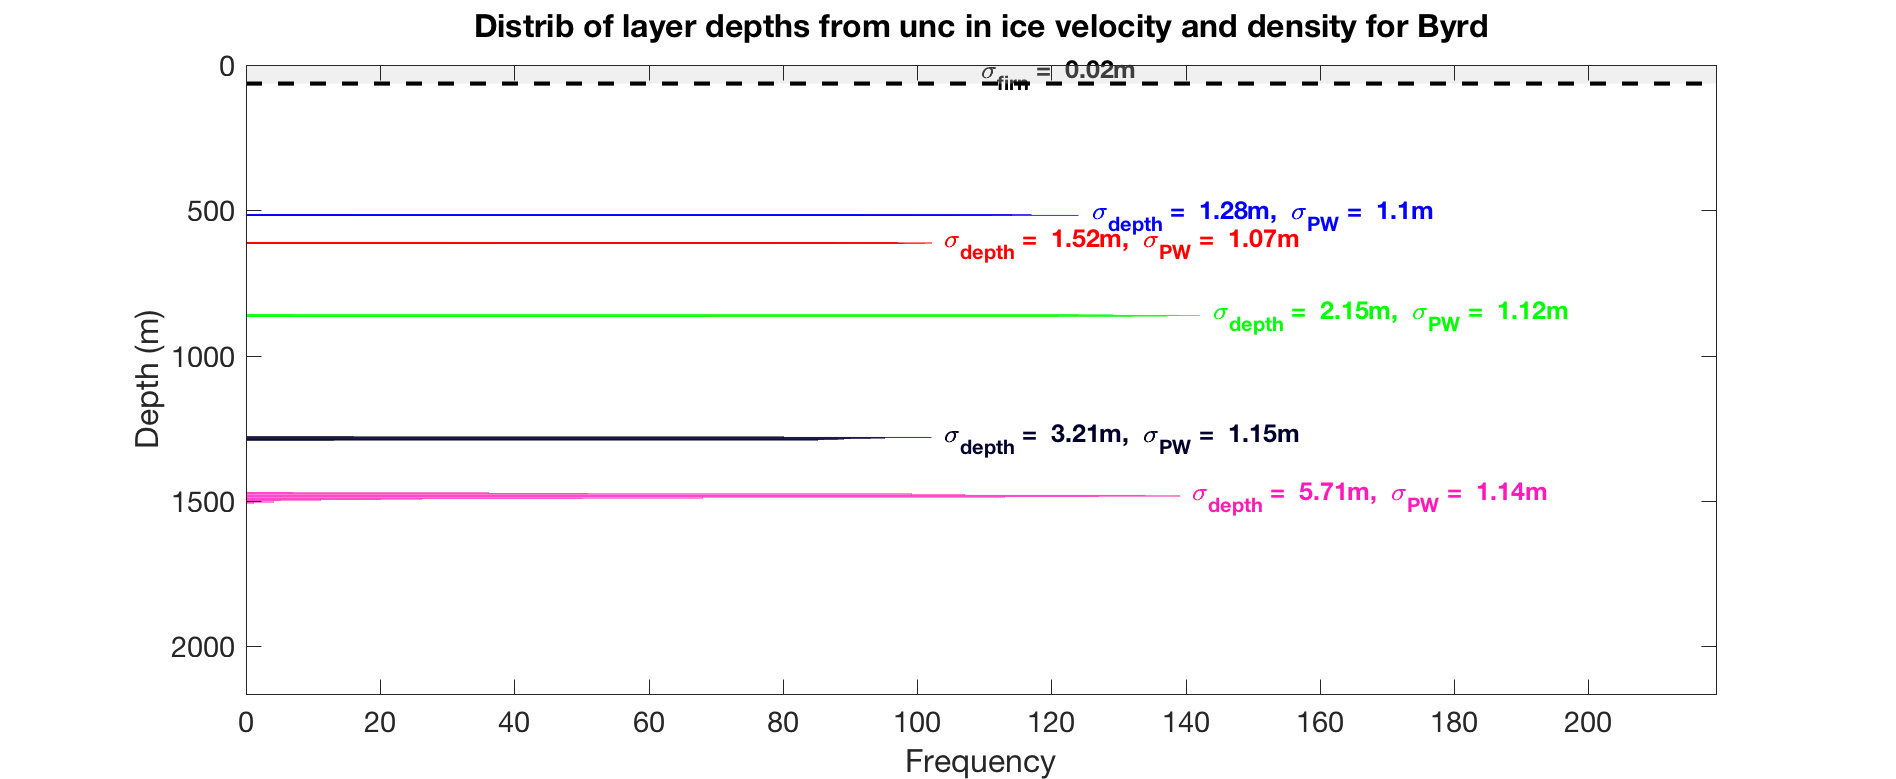
\includegraphics[scale=0.5]{figures/firncorrection}
% %\captionsetup{width=.9\textwidth}
% \caption[]{}
% %\end{center}
% \label{fig:firncorrection}
% \end{figure*}











%Repeat for any additional Supporting audio files

%%% End of body of article:
%%%%%%%%%%%%%%%%%%%%%%%%%%%%%%%%%%%%%%%%%%%%%%%%%%%%%%%%%%%%%%%%
%
% Optional Notation section goes here
%
% Notation -- End each entry with a period.
% \begin{notation}
% Term & definition.\\
% Second term & second definition.\\
% \end{notation}
%%%%%%%%%%%%%%%%%%%%%%%%%%%%%%%%%%%%%%%%%%%%%%%%%%%%%%%%%%%%%%%%


%% ------------------------------------------------------------------------ %%
%%  REFERENCE LIST AND TEXT CITATIONS
%
% Either type in your references using
% \begin{thebibliography}{}
% \bibitem{}
% Text
% \end{thebibliography}
%
% Or,
%
% If you use BiBTeX for your references, please use the agufull08.bst file (available at % ftp://ftp.agu.org/journals/latex/journals/Manuscript-Preparation/) to produce your .bbl
% file and copy the contents into your paper here.
%
% Follow these steps:
% 1. Run LaTeX on your LaTeX file.
%
% 2. Make sure the bibliography style appears as \bibliographystyle{agufull08}. Run BiBTeX on your LaTeX
% file.
%
% 3. Open the new .bbl file containing the reference list and
%   copy all the contents into your LaTeX file here.
%
% 4. Comment out the old \bibliographystyle and \bibliography commands.
%
% 5. Run LaTeX on your new file before submitting.
%
% AGU does not want a .bib or a .bbl file. Please copy in the contents of your .bbl file here.

%\begin{thebibliography}{}

%\providecommand{\natexlab}[1]{#1}
%\expandafter\ifx\csname urlstyle\endcsname\relax
%  \providecommand{\doi}[1]{doi:\discretionary{}{}{}#1}\else
%  \providecommand{\doi}{doi:\discretionary{}{}{}\begingroup
%  \urlstyle{rm}\Url}\fi
%
%\bibitem[{\textit{Atkinson and Sloan}(1991)}]{AtkinsonSloan}
%Atkinson, K., and I.~Sloan (1991), The numerical solution of first-kind
%  logarithmic-kernel integral equations on smooth open arcs, \textit{Math.
%  Comp.}, \textit{56}(193), 119--139.
%
%\bibitem[{\textit{Colton and Kress}(1983)}]{ColtonKress1}
%Colton, D., and R.~Kress (1983), \textit{Integral Equation Methods in
%  Scattering Theory}, John Wiley, New York.
%
%\bibitem[{\textit{Hsiao et~al.}(1991)\textit{Hsiao, Stephan, and
%  Wendland}}]{StephanHsiao}
%Hsiao, G.~C., E.~P. Stephan, and W.~L. Wendland (1991), On the {D}irichlet
%  problem in elasticity for a domain exterior to an arc, \textit{J. Comput.
%  Appl. Math.}, \textit{34}(1), 1--19.
%
%\bibitem[{\textit{Lu and Ando}(2012)}]{LuAndo}
%Lu, P., and M.~Ando (2012), Difference of scattering geometrical optics
%  components and line integrals of currents in modified edge representation,
%  \textit{Radio Sci.}, \textit{47},  RS3007, \doi{10.1029/2011RS004899}.

%\end{thebibliography}

%Reference citation examples:

%...as shown by \textit{Kilby} [2008].
%...as shown by {\textit  {Lewin}} [1976], {\textit  {Carson}} [1986], {\textit  {Bartholdy and Billi}} [2002], and {\textit  {Rinaldi}} [2003].
%...has been shown [\textit{Kilby et al.}, 2008].
%...has been shown [{\textit  {Lewin}}, 1976; {\textit  {Carson}}, 1986; {\textit  {Bartholdy and Billi}}, 2002; {\textit  {Rinaldi}}, 2003].
%...has been shown [e.g., {\textit  {Lewin}}, 1976; {\textit  {Carson}}, 1986; {\textit  {Bartholdy and Billi}}, 2002; {\textit  {Rinaldi}}, 2003].

%...as shown by \citet{jskilby}.
%...as shown by \citet{lewin76}, \citet{carson86}, \citet{bartoldy02}, and \citet{rinaldi03}.
%...has been shown \citep{jskilbye}.
%...has been shown \citep{lewin76,carson86,bartoldy02,rinaldi03}.
%...has been shown \citep [e.g.,][]{lewin76,carson86,bartoldy02,rinaldi03}.
%
% Please use ONLY \citet and \citep for reference citations.
% DO NOT use other cite commands (e.g., \cite, \citeyear, \nocite, \citealp, etc.).

%% ------------------------------------------------------------------------ %%
%
%  END ARTICLE
%
%% ------------------------------------------------------------------------ %%
\end{article}
\clearpage

% Delete all unused file types below. Copy/paste for multiples of each file type as needed.

% enter figures and tables here:
%
% EXAMPLE FIGURE
% ---------------
% \begin{figure}
%\setfigurenum{S1} %%Change number for each figure
% \noindent\includegraphics[width=20pc]{samplefigure.eps}
%\caption{Caption text here}
 %\label{figure_label}
 %\end{figure}

% ---------------
% EXAMPLE TABLE
%
%\begin{table}
%\settablenum{S1} %%Change number for each table
%\caption{Time of the Transition Between Phase 1 and Phase 2\tablenotemark{a}}
%\centering
%\begin{tabular}{l c}
%\hline
% Run  & Time (min)  \\
%\hline
%  $l1$  & 260   \\
%  $l2$  & 300   \\
%  $l3$  & 340   \\
%  $h1$  & 270   \\
%  $h2$  & 250   \\
%  $h3$  & 380   \\
%  $r1$  & 370   \\
%  $r2$  & 390   \\
%\hline
%\end{tabular}
%\tablenotetext{a}{Footnote text here.}
%\end{table}
% ---------------
%
% EXAMPLE LARGE TABLE (UPLOADED SEPARATELY)
%\begin{table}
%\settablenum{S1} %%Change number for each table
%\caption{Time of the Transition Between Phase 1 and Phase 2\tablenotemark{a}}
%\end{table}


\end{document}

%%%%%%%%%%%%%%%%%%%%%%%%%%%%%%%%%%%%%%%%%%%%%%%%%%%%%%%%%%%%%%%

More Information and Advice:

%% ------------------------------------------------------------------------ %%
%
%  SECTION HEADS
%
%% ------------------------------------------------------------------------ %%

% Capitalize the first letter of each word (except for
% prepositions, conjunctions, and articles that are
% three or fewer letters).

% AGU follows standard outline style; therefore, there cannot be a section 1 without
% a section 2, or a section 2.3.1 without a section 2.3.2.
% Please make sure your section numbers are balanced.
% ---------------
% Level 1 head
%
% Use the \section{} command to identify level 1 heads;
% type the appropriate head wording between the curly
% brackets, as shown below.
%
%An example:
%\section{Level 1 Head: Introduction}
%
% ---------------
% Level 2 head
%
% Use the \subsection{} command to identify level 2 heads.
%An example:
%\subsection{Level 2 Head}
%
% ---------------
% Level 3 head
%
% Use the \subsubsection{} command to identify level 3 heads
%An example:
%\subsubsection{Level 3 Head}
%
%---------------
% Level 4 head
%
% Use the \subsubsubsection{} command to identify level 3 heads
% An example:
%\subsubsubsection{Level 4 Head} An example.
%
%% ------------------------------------------------------------------------ %%
%
%  IN-TEXT LISTS
%
%% ------------------------------------------------------------------------ %%
%
% Do not use bulleted lists; enumerated lists are okay.
% \begin{enumerate}
% \item
% \item
% \item
% \end{enumerate}
%
%% ------------------------------------------------------------------------ %%
%
%  EQUATIONS
%
%% ------------------------------------------------------------------------ %%

% Single-line equations are centered.
% Equation arrays will appear left-aligned.

Math coded inside display math mode \[ ...\]
 will not be numbered, e.g.,:
 \[ x^2=y^2 + z^2\]

 Math coded inside \begin{equation} and \end{equation} will
 be automatically numbered, e.g.,:
 \begin{equation}
 x^2=y^2 + z^2
 \end{equation}

% IF YOU HAVE MULTI-LINE EQUATIONS, PLEASE
% BREAK THE EQUATIONS INTO TWO OR MORE LINES
% OF SINGLE COLUMN WIDTH (20 pc, 8.3 cm)
% using double backslashes (\\).

% To create multiline equations, use the
% \begin{eqnarray} and \end{eqnarray} environment
% as demonstrated below.
\begin{eqnarray}
  x_{1} & = & (x - x_{0}) \cos \Theta \nonumber \\
        && + (y - y_{0}) \sin \Theta  \nonumber \\
  y_{1} & = & -(x - x_{0}) \sin \Theta \nonumber \\
        && + (y - y_{0}) \cos \Theta.
\end{eqnarray}

%If you don't want an equation number, use the star form:
%\begin{eqnarray*}...\end{eqnarray*}

% Break each line at a sign of operation
% (+, -, etc.) if possible, with the sign of operation
% on the new line.

% Indent second and subsequent lines to align with
% the first character following the equal sign on the
% first line.

% Use an \hspace{} command to insert horizontal space
% into your equation if necessary. Place an appropriate
% unit of measure between the curly braces, e.g.
% \hspace{1in}; you may have to experiment to achieve
% the correct amount of space.


%% ------------------------------------------------------------------------ %%
%
%  EQUATION NUMBERING: COUNTER
%
%% ------------------------------------------------------------------------ %%

% You may change equation numbering by resetting
% the equation counter or by explicitly numbering
% an equation.

% To explicitly number an equation, type \eqnum{}
% (with the desired number between the brackets)
% after the \begin{equation} or \begin{eqnarray}
% command.  The \eqnum{} command will affect only
% the equation it appears with; LaTeX will number
% any equations appearing later in the manuscript
% according to the equation counter.
%

% If you have a multiline equation that needs only
% one equation number, use a \nonumber command in
% front of the double backslashes (\\) as shown in
% the multiline equation above.

%% ------------------------------------------------------------------------ %%
%
%  SIDEWAYS FIGURE AND TABLE EXAMPLES
%
%% ------------------------------------------------------------------------ %%
%
% For tables and figures, add \usepackage{rotating} to the paper and add the rotating.sty file to the folder.
% AGU prefers the use of {sidewaystable} over {landscapetable} as it causes fewer problems.
%
% \begin{sidewaysfigure}
% \includegraphics[width=20pc]{samplefigure.eps}
% \caption{caption here}
% \label{label_here}
% \end{sidewaysfigure}
%
%
%
% \begin{sidewaystable}
% \caption{}
% \begin{tabular}
% Table layout here.
% \end{tabular}
% \end{sidewaystable}
%
%

